\documentclass[11pt,a4paper]{article}

\usepackage[margin=22mm]{geometry}
\usepackage{amsmath,amssymb}
\usepackage{booktabs}
\usepackage{graphicx}
\usepackage{float}
\usepackage{xcolor}
\usepackage[hidelinks]{hyperref}
\usepackage{microtype}

\definecolor{BPHOBlue}{HTML}{0072B2}
\definecolor{BPHOGreen}{HTML}{009E73}
\definecolor{BPHOText}{HTML}{172033}
\graphicspath{{../../figures/task07/}}

\title{\textbf{Particle in a One-Dimensional Box}\\
\large Energy Quantisation, Probability Density and Heisenberg Uncertainty}
\author{BPhO Computational Challenge 2026 --- Task 7}
\date{}

\begin{document}
\maketitle

\begin{abstract}
This report implements the exact stationary states of a non-relativistic
particle confined by an infinite one-dimensional potential well.  The energy
spectrum and Born probability densities satisfy the official Task~7
requirements.  The extension evaluates the position and momentum moments and
shows analytically and computationally that every state obeys
$\Delta x\Delta p\geq\hbar/2$.  A finite-difference eigensolver provides an
independent numerical check of the analytical solution.
\end{abstract}

\section{Physical model}

The potential is zero inside a box of width $a$ and infinite outside:
\begin{equation}
V(x)=
\begin{cases}
0, & 0<x<a,\\
\infty, & x\leq0\text{ or }x\geq a.
\end{cases}
\end{equation}
The wavefunction must therefore vanish at both walls,
$\psi(0)=\psi(a)=0$.  Within the box the time-independent Schr\"odinger
equation is
\begin{equation}
-\frac{\hbar^2}{2m}\frac{d^2\psi}{dx^2}=E\psi.
\end{equation}
The boundary conditions select positive integer quantum numbers
$n=1,2,\ldots$ and normalized eigenstates
\begin{equation}
\psi_n(x,t)=\sqrt{\frac{2}{a}}
\sin\!\left(\frac{n\pi x}{a}\right)e^{-iE_nt/\hbar}.
\end{equation}
The corresponding energy spectrum is
\begin{equation}
E_n=\frac{n^2\pi^2\hbar^2}{2ma^2}
=\frac{n^2h^2}{8ma^2}.
\label{eq:energy}
\end{equation}
The computational baseline uses an electron and $a=1.00\,\mathrm{nm}$.

\section{Probability density}

The Born probability density is
\begin{equation}
|\psi_n(x,t)|^2=\frac{2}{a}
\sin^2\!\left(\frac{n\pi x}{a}\right).
\end{equation}
The factor $e^{-iE_nt/\hbar}$ has unit modulus, so a single energy eigenstate
has a time-independent probability density.  Normalisation follows from
\begin{equation}
\int_0^a |\psi_n|^2\,dx
=\frac{2}{a}\int_0^a\sin^2\!\left(\frac{n\pi x}{a}\right)dx=1.
\end{equation}
State $n$ has $n-1$ interior nodes at $x=ka/n$, where
$k=1,\ldots,n-1$.

\begin{figure}[H]
\centering
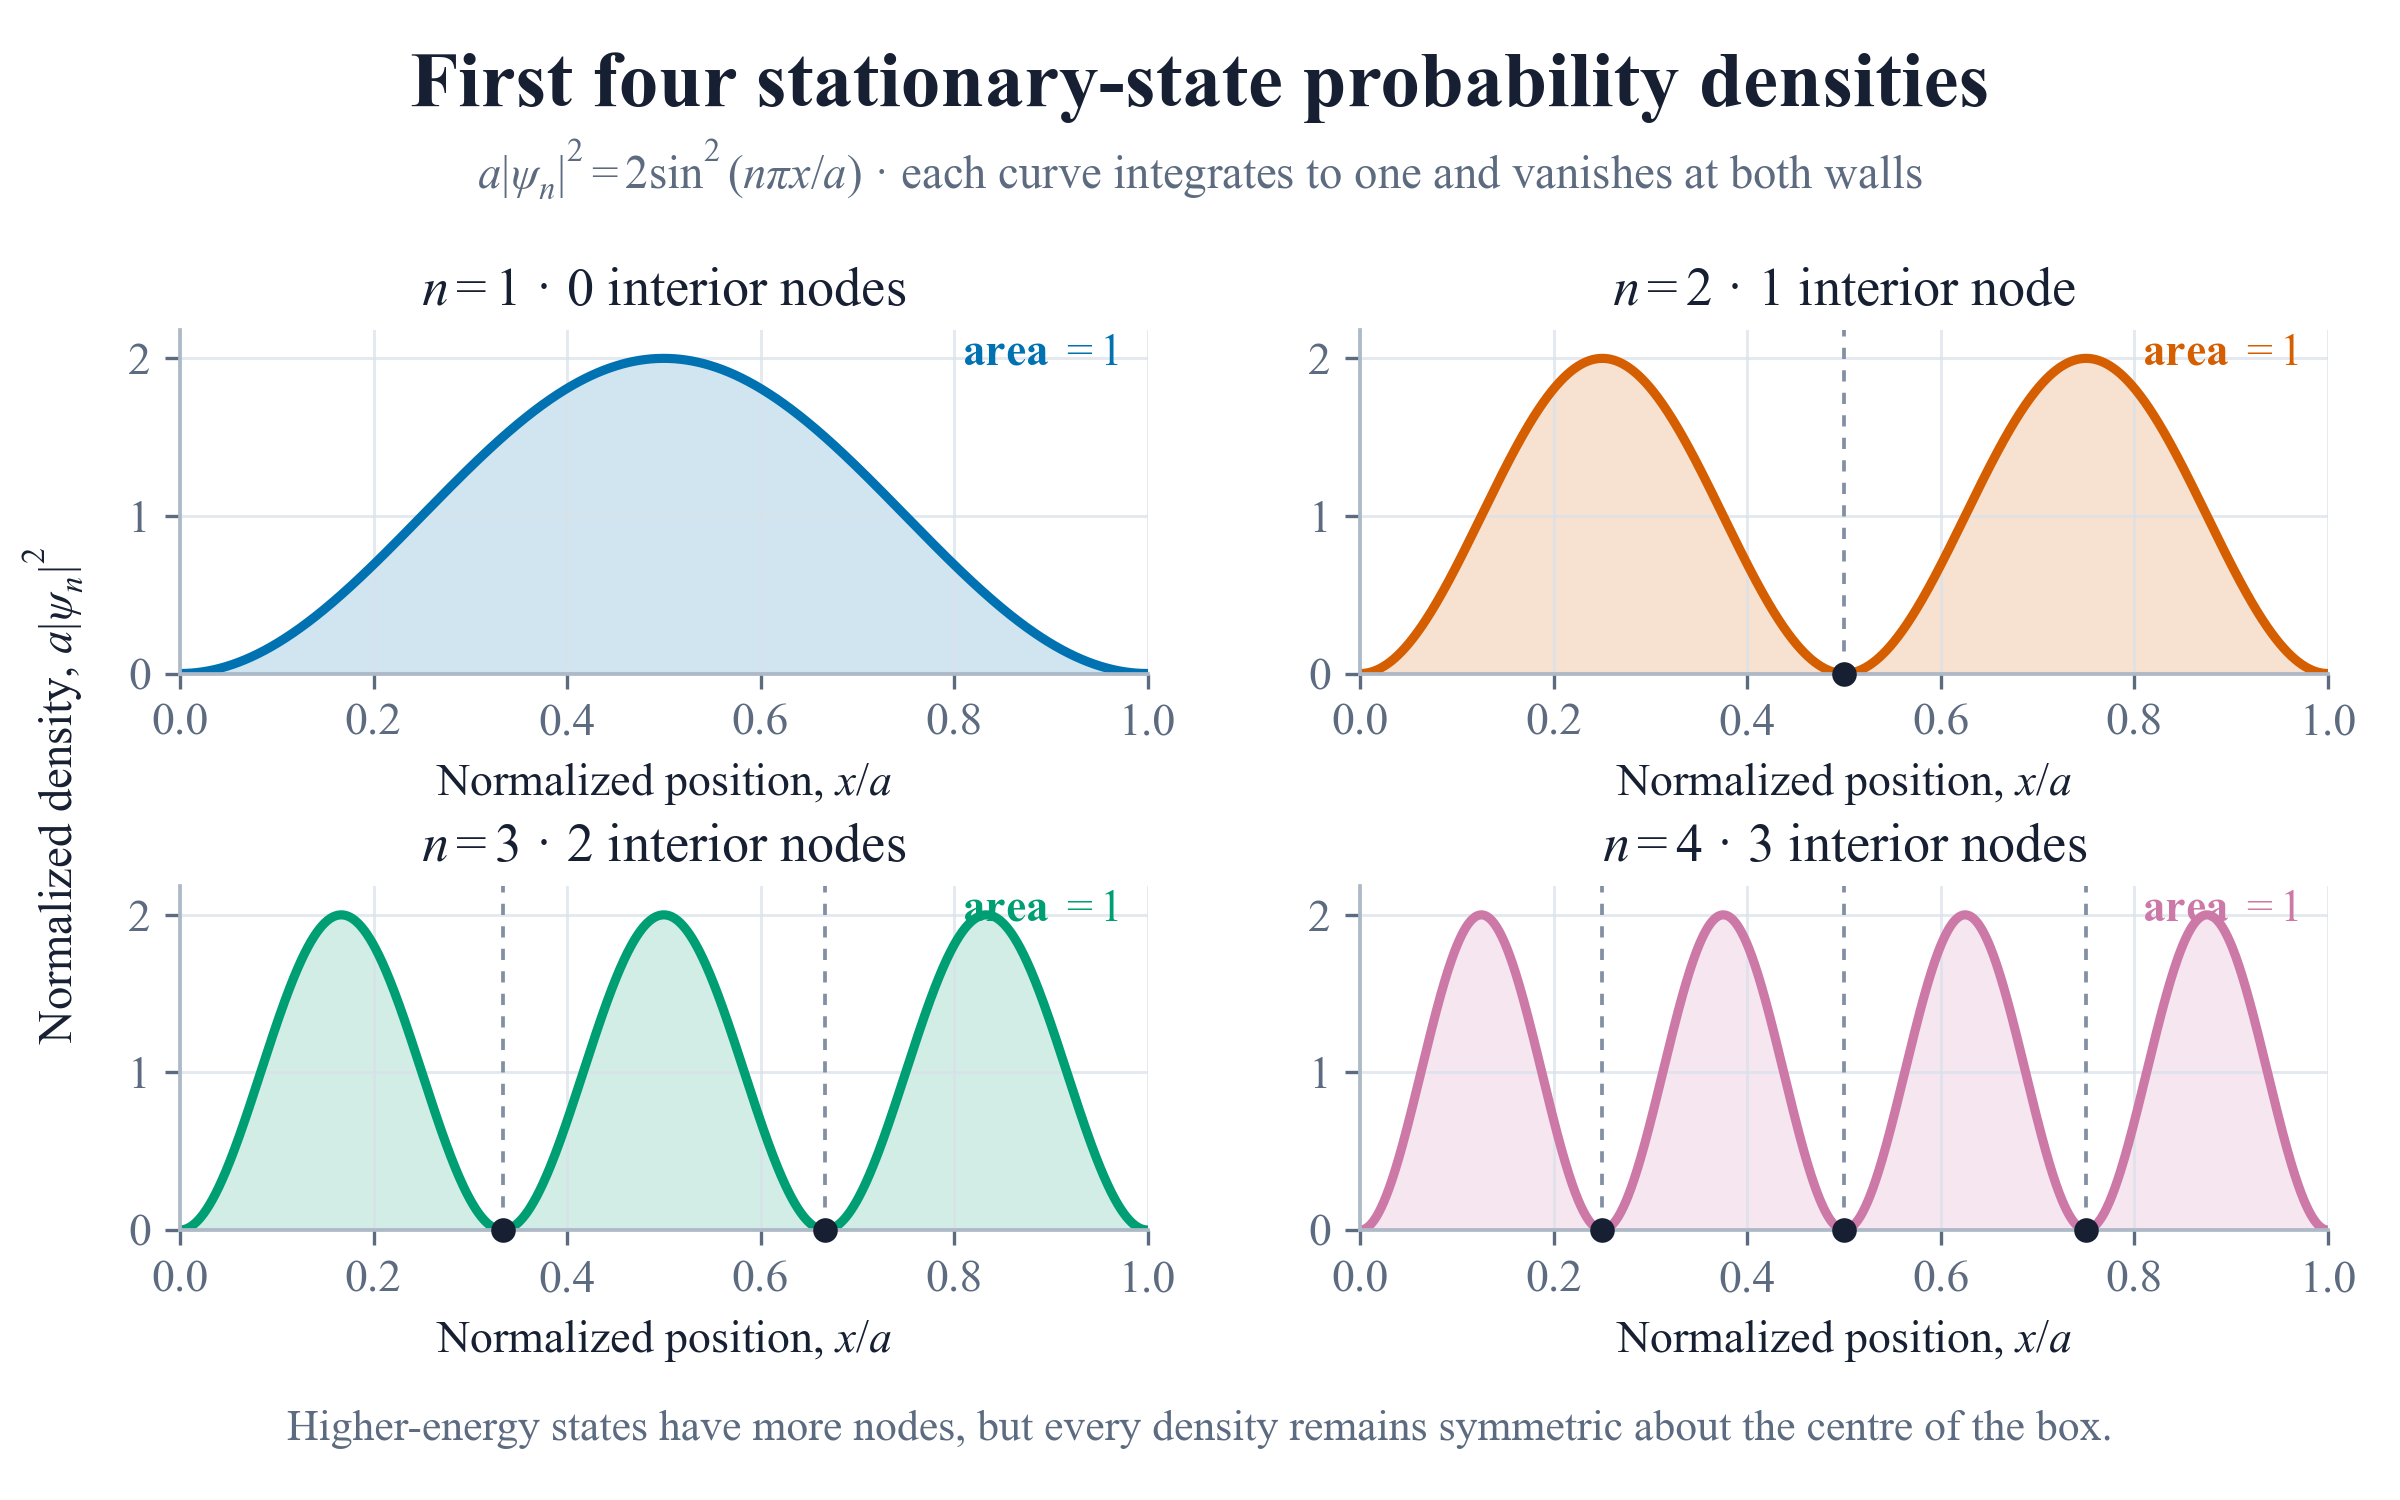
\includegraphics[width=0.92\textwidth]{probability_densities.png}
\caption{Dimensionless probability densities for the first four stationary
states.  The area under every curve is one.}
\end{figure}

\section{Position uncertainty}

The expectation value of position is
\begin{equation}
\langle x\rangle
=\int_0^a x|\psi_n|^2\,dx=\frac{a}{2}.
\end{equation}
The second moment is
\begin{align}
\langle x^2\rangle
&=\frac{2}{a}\int_0^a x^2
\sin^2\!\left(\frac{n\pi x}{a}\right)dx\\
&=a^2\left(\frac{1}{3}-\frac{1}{2n^2\pi^2}\right).
\end{align}
Consequently,
\begin{align}
(\Delta x)^2
&=\langle x^2\rangle-\langle x\rangle^2\\
&=a^2\left(\frac{1}{12}-\frac{1}{2n^2\pi^2}\right),
\end{align}
and
\begin{equation}
\Delta x=a\sqrt{\frac{1}{12}-\frac{1}{2n^2\pi^2}}.
\label{eq:delta-x}
\end{equation}

\section{Momentum uncertainty}

The momentum operator is
\begin{equation}
\hat p=-i\hbar\frac{d}{dx}.
\end{equation}
Because each spatial eigenfunction is real and vanishes at the boundaries,
\begin{align}
\langle p\rangle
&=\int_0^a\psi_n^*\left(-i\hbar\frac{d}{dx}\right)\psi_n\,dx\\
&=-\frac{i\hbar}{2}\left[\psi_n^2\right]_0^a=0.
\end{align}
Applying the momentum operator twice gives
\begin{align}
\langle p^2\rangle
&=\int_0^a\psi_n^*\left(-\hbar^2\frac{d^2}{dx^2}\right)\psi_n\,dx\\
&=\frac{n^2\pi^2\hbar^2}{a^2}.
\end{align}
Thus
\begin{equation}
\Delta p=\sqrt{\langle p^2\rangle-\langle p\rangle^2}
=\frac{n\pi\hbar}{a}.
\label{eq:delta-p}
\end{equation}

\section{Verification of the uncertainty principle}

Multiplying Eqs.~\eqref{eq:delta-x} and \eqref{eq:delta-p} gives
\begin{equation}
\boxed{
\Delta x\Delta p
=\hbar\sqrt{\frac{n^2\pi^2}{12}-\frac{1}{2}}
}.
\label{eq:uncertainty-product}
\end{equation}
The expression increases with positive integer $n$, so its minimum occurs at
$n=1$:
\begin{equation}
\frac{\Delta x\Delta p}{\hbar}
=\sqrt{\frac{\pi^2}{12}-\frac{1}{2}}
=0.567861808\ldots > \frac{1}{2}.
\end{equation}
Therefore every stationary state in the box satisfies Heisenberg's relation
\begin{equation}
\Delta x\Delta p\geq\frac{\hbar}{2}.
\end{equation}
The box ground state is not a minimum-uncertainty Gaussian state, so the
inequality is strict.

\begin{figure}[H]
\centering
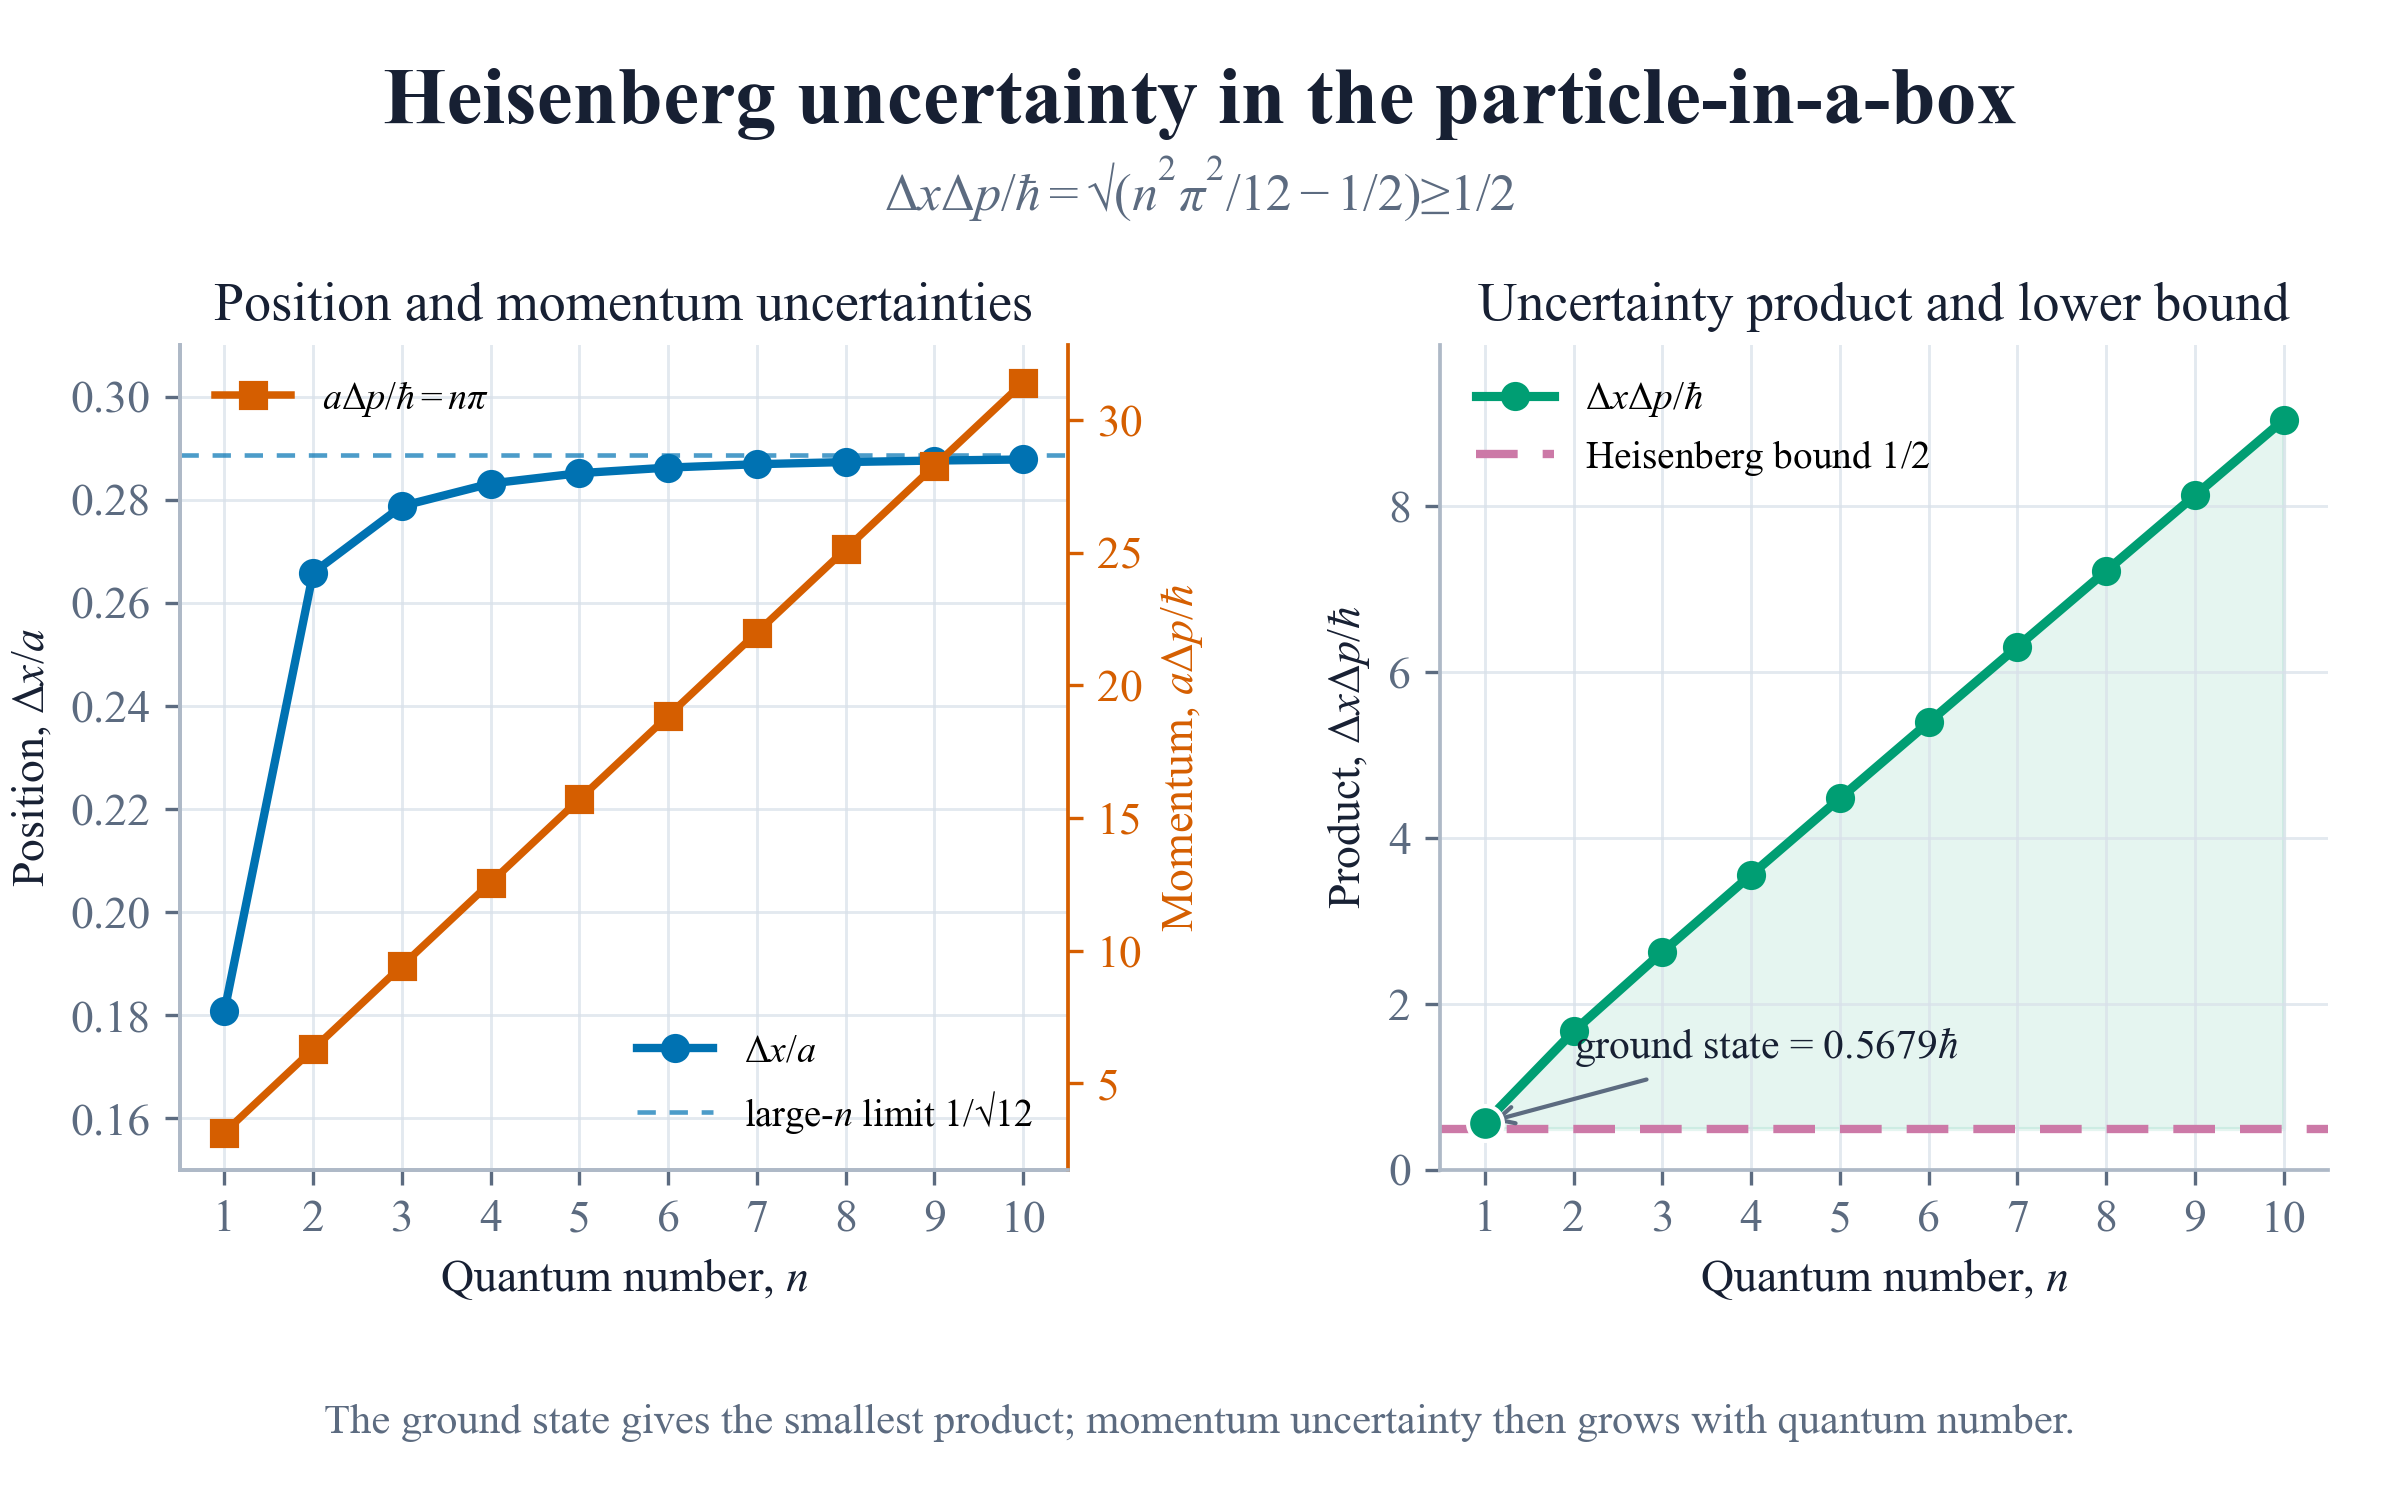
\includegraphics[width=0.90\textwidth]{uncertainty_principle.png}
\caption{Position and momentum uncertainties and their product for
$n=1,\ldots,10$.  The dashed magenta line marks the Heisenberg bound.}
\end{figure}

\section{Computational implementation and validation}

The analytical model evaluates Eqs.~\eqref{eq:energy}--
\eqref{eq:uncertainty-product} on a 2001-point position grid.  A separate
finite-difference model approximates the second derivative by
\begin{equation}
\left.\frac{d^2\psi}{dx^2}\right|_j
\approx\frac{\psi_{j+1}-2\psi_j+\psi_{j-1}}{(\Delta x)^2},
\end{equation}
creating a symmetric tridiagonal Hamiltonian.  Its eigenvalues are calculated
without inserting the analytical spectrum.  Position and momentum moments are
then computed directly from each normalized numerical eigenvector using
\begin{equation}
\langle A\rangle_h=\sum_j\psi_j^*(A_h\psi)_j\,\Delta x,
\qquad
(p_h\psi)_j=-i\hbar\frac{\psi_{j+1}-\psi_{j-1}}{2\Delta x}.
\end{equation}
The same zero-valued boundary points used by the Hamiltonian close the
first- and second-derivative stencils.  Analytical uncertainties are introduced
only after the numerical $\langle x\rangle$, $\langle x^2\rangle$,
$\langle p\rangle$ and $\langle p^2\rangle$ have been evaluated.

\begin{table}[H]
\centering
\caption{Maximum relative energy error over the first ten numerical states.}
\begin{tabular}{rr}
\toprule
Interior points & Maximum relative error\\
\midrule
100  & $8.04\times10^{-3}$\\
200  & $2.03\times10^{-3}$\\
400  & $5.11\times10^{-4}$\\
800  & $1.28\times10^{-4}$\\
1600 & $3.21\times10^{-5}$\\
\bottomrule
\end{tabular}
\end{table}

For $N=1600$, the maximum relative errors in $\Delta p$ and
$\Delta x\Delta p$ are both below $1.605\times10^{-5}$.  Their measured
convergence orders over all ten states lie between 1.99961 and 2.00038,
consistent with second-order discretisation.  The energy orders lie between
1.99896 and 1.99996.  The finest-grid absolute
overlap between every numerical eigenvector and its analytical counterpart is
greater than 0.999999.  All fifty grid--state uncertainty products satisfy
$\Delta x\Delta p\geq\hbar/2$.  The 50-check acceptance suite additionally checks
normalisation, orthogonality, node counts, boundary values, energy scaling,
expectation values and the uncertainty inequality.

\section{Interpretation and limitations}

The infinite well is an ideal model: real confining potentials are finite and
may allow tunnelling.  The calculation is one-dimensional, non-relativistic
and contains one non-interacting particle with no external field or spin
dynamics.  These assumptions do not affect the internal verification of the
specified Task~7 model, but they limit direct quantitative comparison with a
particular laboratory system.

\paragraph{Reproducibility.}
The source code, CSV evidence, reference anchors, validation report, PNG/SVG
figures and deterministic manifest are generated by a single command.  The
official brief is available from the
\href{https://www.bpho.org.uk/bpho/computational-challenge/}{British Physics
Olympiad Computational Challenge page}.

\end{document}
